% \documentclass[handout,hyperref={pdfpagelabels=false},aspectratio=169]{beamer} % print pdf without pause (overleaf specification)
\documentclass[hyperref={pdfpagelabels=false},aspectratio=169]{beamer}
\usepackage{booktabs} % Allows the use of \toprule, \midrule and \bottomrule for better rules in tables
\usepackage{calligra} % Font for wordart
\usepackage{appendixnumberbeamer}
\usepackage{listings} % For code display
\usepackage{multirow}
\usepackage{graphicx}
\usepackage{float}
\usepackage{booktabs}
\usepackage{tikz}
\usepackage{array}
\usepackage[utf8x]{inputenc}
\usepackage{url}
\usepackage{setspace}
\usepackage{hyperref}
\usepackage{amsmath}
\setlength{\parskip}{3pt}
\setbeamertemplate{caption}[numbered]{}% Number float-like environments




%---------------------------------------------------------
%	CITATIONS / REFERENCES
%---------------------------------------------------------
\usepackage[style=apa,backend=biber]{biblatex}
\addbibresource{bib.bib}
%\bibliographystyle{apalike}



%---------------------------------------------------------
%	SELECT THEME & COLORS
%---------------------------------------------------------
\usetheme{Madrid}
\definecolor{MonashBlue}{RGB}{0, 99, 167}
\definecolor{Orange}{RGB}{204, 89, 0}

\setbeamercolor*{structure}{bg=MonashBlue, fg=MonashBlue}
% Title block and bottom right box color
\setbeamercolor*{palette primary}{use=structure, fg=white,bg=MonashBlue}
% Bottom left box and bar between title & top bubbles
\setbeamercolor*{palette secondary}{use=structure, fg=MonashBlue, bg=white}
% Probably not used
\setbeamercolor*{palette tertiary}{use=structure, fg=white, bg=MonashBlue} 

% Title of each slide
\setbeamercolor{frametitle}{bg=MonashBlue, fg=white}
\setbeamercolor*{titlelike}{parent=palette primary}


%%% Headline and Central Footer %%%
% You can change the theme back and forth for each frame

% Theme II - gold head, gold foot (as shown in the title frame)
    \setbeamercolor{section in head/foot}{fg=white, bg=Orange}
    \setbeamercolor{headline}{fg=white, bg=Orange}



%%% Specific Colors %%%
\setbeamercolor{item projected}{bg=Orange}
\setbeamertemplate{enumerate items}{bg=Orange}

\setbeamercolor{itemize item}{fg=Orange}
\setbeamercolor{itemize subitem}{fg=Orange}

\setbeamercolor{button}{bg=Orange}

%%% Edits ONLY the TOC slide %%%
\setbeamercolor{section in toc}{fg=black}
\setbeamercolor{subsection in toc}{fg=black}

%%% Block Colors %%%
% Standard block
    \setbeamercolor{block title}{bg=Orange, fg=white}
    \setbeamercolor{block body}{bg=Orange!20}
% Alerted block
    \setbeamercolor{block title alerted}{bg=orange, fg=white}
    \setbeamercolor{block body alerted}{bg=orange!10}
% Example block
    \setbeamercolor{block title example}{bg=MonashBlue, fg=white}
    \setbeamercolor{block body example}{bg=MonashBlue!10}

%---------------------------------------------------------
%	SELECT THE FONT THEME & FONTS
%---------------------------------------------------------
\usefonttheme{default} % Typeset using the default sans serif font
\usepackage{palatino} % Use the Palatino font for serif text
\usepackage[default]{opensans} % Use the Open Sans font for sans serif text
\useinnertheme{circles}

%---------------------------------------------------------
%	SELECT THE OUTER THEME
%---------------------------------------------------------

% \useoutertheme{default}
% \useoutertheme{miniframes}
% \useoutertheme{infolines}
% \useoutertheme{smoothbars}
% \useoutertheme{sidebar}
 \useoutertheme{split}
% \useoutertheme{shadow}
% \useoutertheme{tree}
% \useoutertheme{smoothtree}

%---------------------------------------------------------
%	PRESENTATION INFORMATION
%---------------------------------------------------------

\title[Revisiting Forecast Combination Puzzle]{Revisiting Forecast Combination Puzzle}
% Click the middle footer can switch between the first and last numbered frame
\subtitle{An Empirical Study}

\author[Honours Preliminary Presentation]{\Large{XIEFEI (SAPPHIRE) LI}}
\institute[]{Department of Econometrics and Business Statistics \\ 

\textit{xlii0145@student.monash.edu} \\ \bigskip
\text{\small{Supervisor: David T. Frazier}}
}
\date[May 2023]

\logo{
\includegraphics[width=2.5cm]{Graph/Monash.png}}

%---------------------------------------------------------
%	CODE DISPLAY
%---------------------------------------------------------
\lstset{
    basicstyle=\ttfamily\small,
    keywordstyle=\bfseries\color{blue},
    emphstyle=\ttfamily\color{red},   
    stringstyle=\color{green},
    numbers=left,
    numberstyle=\small\color{gray},
    rulesepcolor=\color{red!20!green!20!blue!20},
    frame=shadowbox,
    xleftmargin=1cm,
    xrightmargin=1cm,
}

%---------------------------------------------------------
%	EXTRA SETTINGS
%---------------------------------------------------------

% Clear warnings related to \translate
%     https://github.com/josephwright/beamer/issues/449
\pdfstringdefDisableCommands{
    \def\translate#1{#1}
}

% Adjust header height
\setbeamertemplate{headline}{
    \nointerlineskip
    \begin{beamercolorbox}[wd=\paperwidth,ht=7.0ex]{headline}
        \insertnavigation{\paperwidth}\vspace*{2.0ex}
    \end{beamercolorbox}
}

% Disable navigation symbols
\setbeamertemplate{navigation symbols}{}
\setbeamersize
{
    text margin left=1cm,
    text margin right=1cm
}

%---------------------------------------------------------
%   DOCUMENT BEGINS
%---------------------------------------------------------
\begin{document}

%---------------------------------------------------------
%	TITLE SLIDE
%---------------------------------------------------------
\section{}

\begin{frame}
\titlepage % Output the title slide, automatically created using the text entered in the PRESENTATION INFORMATION block above
\end{frame}

% Clear background
\usebackgroundtemplate{}



\setbeamercolor{section in head/foot}{fg=Orange, bg=white}
\setbeamercolor{headline}{fg=Orange, bg=white}

\section{Motivation}

\logo{}

\begin{frame}{Forecast combination - point and density}

    Combining multiple forecasts can dramatically improve the accuracy of the forecast (\cite{BG69}).
    
    \vspace{5mm}

    
    Point Forecast Combination 
    \[\hat y_t = \omega \ \hat y_{1t} + (1-\omega) \ \hat y_{2t}\]

    Density Forecast Combination
    \[ \hat f(y_t) = \omega \ \hat f_1(y_t) + (1-\omega) \hat f_2(y_t)\]

\end{frame}


\begin{frame}{Forecast combination puzzle}

\begin{columns}[t]
    \begin{column}{0.5\textwidth}
        \centering
        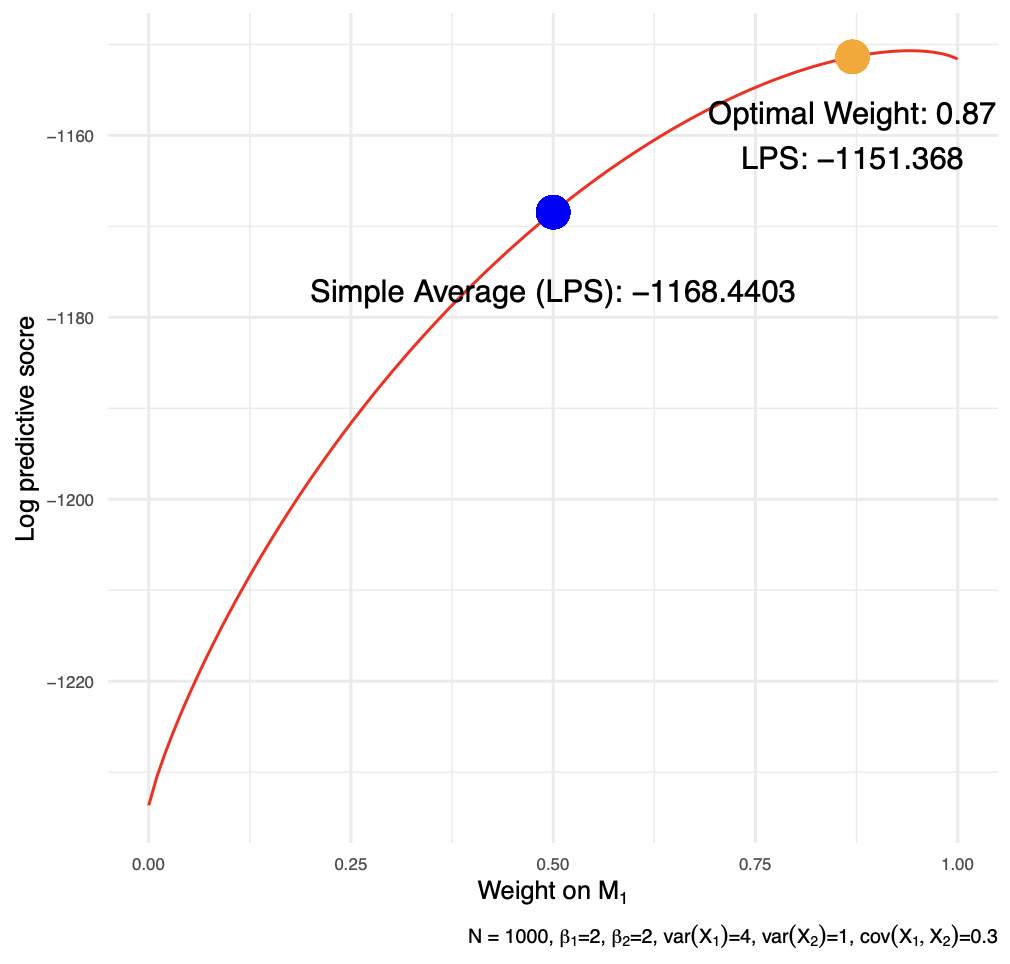
\includegraphics[width=6cm]{Graph/Ex1.png}
    \end{column}
    
    \begin{column}{0.5\textwidth}
        \centering
        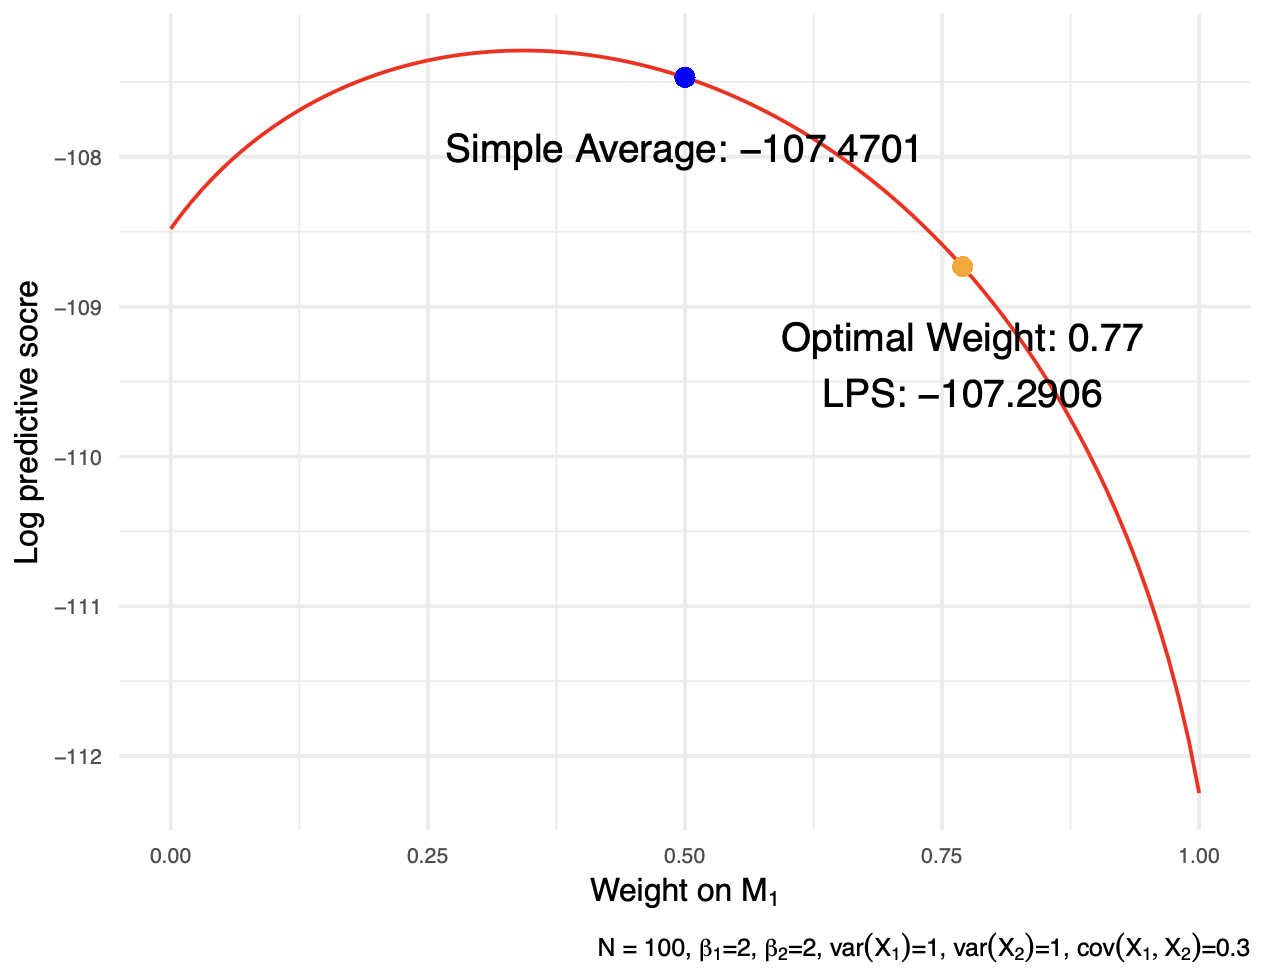
\includegraphics[width=6cm]{Graph/Ex2.png}
    \end{column}
    \end{columns}

    \vspace{-6mm}
    
    \begin{columns}[t]
    \begin{column}{0.5\textwidth}
        \begin{alertblock}{}
        \centering
        \tikz{\fill[orange] circle (3pt);} \ Complicated Weighting Schemes
        \end{alertblock}
    \end{column}
    
    \begin{column}{0.5\textwidth}
        \begin{exampleblock}{}
        \centering
        \tikz{\fill[blue] circle (3pt);} \ Simple Averaging
        / Equal Weights
        \end{exampleblock}
    \end{column}
    \end{columns}

\end{frame}



\begin{frame}{When should we expect the puzzle}

    In the linear regression context, the optimal weight $\hat\omega_{opt}$ has a closed-form expression when using the Mean Squared Error (MSE) weighting scheme.
    
    
    \[\hat\omega_{opt} \overset{p}{\to} \omega_\star = \frac{\alpha_1'\Sigma_{11}\alpha_1 - \alpha_1'\Sigma_{12}\alpha_2}{\alpha_1'\Sigma_{11}\alpha_1 - 2\alpha_1'\Sigma_{12}\alpha_2 + \alpha_2'\Sigma_{22}\alpha_2}\]


    The presence of the puzzle is tightly related to the coefficients and the variances of regressors in both proposed models.
    
    
    \[\omega_\star=\frac{1}{2} \Rightarrow \alpha_1'\Sigma_{11}\alpha_1 = \alpha_2'\Sigma_{22}\alpha_2\]

    In-sample performance

    
\end{frame}



\begin{frame}{Preliminary Conjecture}

    Consider a two-model combination.

    \begin{table}[ht]
    \centering
    \begin{tabular}{cccc}
                           &      & \multicolumn{2}{c}{$M_2$} \\
                           &      & Good       & Bad       \\
    \multirow{2}{*}{$M_1$} & Good & \alt<2>{\color{MonashBlue} $\surd$}{$\surd$}    & \alt<2>{\color{Orange} $?$}{$?$} \\
                           & Bad  & \alt<2>{\color{Orange} $?$}{$?$}        & \alt<2>{\color{MonashBlue} $\surd$}{$\surd$}
    \end{tabular}
    \label{tab:1}
    \caption{\footnotesize Initial conjecture on the presence of forecast combination puzzle}
    \end{table}
    
    The in-sample fit between two models in a relative sense may indicate the presence of the puzzle.


\end{frame}



\begin{frame}{Preliminary Conjecture}
\centering
\begin{tikzpicture}
    \draw[step=1cm,gray,very thin];
    \draw[thick,->] (0,0) -- (7,0);
    \draw[thick,->] (0,0) -- (0,5);
    \draw[thick,->] (0,0) -- (7,0) node[anchor=north west] {$M_1$ LogL};
    \draw[thick,->] (0,0) -- (0,5) node[anchor=south east] {$M_2$ LogL};
    
    \foreach \Point in {(1,1), (2,2), (3,3), (4,4)}{
    \node [MonashBlue] at \Point {$\surd$};}
    
    \foreach \Point in {(6,2), (5,1), (1,4), (2,5)}{
    \node [Orange] at \Point {$?$};}

    \foreach \Point/\PointLabel in {(6,2)/GB, (5,1)/GB, (1,4)/BG, (2,5)/BG}
        \draw[fill=Orange] \Point circle (0.0005) node[above right] {\color{Orange} \PointLabel};
\end{tikzpicture}

\end{frame}







\section{Background}


\begin{frame}
    \frametitle{Explanations of the puzzle in literature}

        \begin{exampleblock}{\large{Uncertainty in Weight Estimation}}
        The simple averaging does not require any estimation (\cite{SW98}, \cite{SW04}, and \cite{SW09}).
        \end{exampleblock}

        \vspace{4mm}

        \begin{exampleblock}{\large{Trade-off between Bias and Variance}}
        The equally weighted combination is unbiased and its variance has only one component (\cite{E11} and \cite{CMVW16}).
        \end{exampleblock}

\end{frame}




\begin{frame}
\frametitle{A Recent (General) Explanation}

    \begin{exampleblock}{\large{Estimation Uncertainty on Forecast Performance}}
    Asymptotically, the bias and sampling variability mainly come from the estimation of the models used to produce the constituent model forecasts (\cite{ZMFP22} and \cite{FZMP23}).
    \end{exampleblock}

    \vspace{4mm}
    
    These explanations all implicitly assume that \textbf{the puzzle will be in evidence} when combining forecasts, regardless of the choice of constituent models or the weighing scheme. 


\end{frame}


\begin{frame}{Research Gap}
    
    Forecast combination has attracted wide attention and contributions in the literature, both theoretical and applied (\cite{C89} and \cite{T06}).

    \vspace{4mm}
    
    Researchers have examined a variety of combination methods for both point and density forecasts over the past 50 years, see \cite{WHLK22} for a modern literature review.

    \vspace{4mm}
    
    No attention appears to have been given to \textbf{the cross-sectional setting}. 
    
\end{frame}


\begin{frame}
    \frametitle{Research objectives}

    \begin{enumerate}[<+->]
        \item To \textbf{substantiate the presence} of the combination puzzle in the time series setting with empirical data. \newline
        \item To systematically investigate the determinants behind, and evidence for, the \textbf{forecast combination puzzle in the cross-sectional setting} using simulated data. \newline
        \item To \textbf{validate our preliminary conjecture} with empirical evidence.
    \end{enumerate}

\end{frame}



\section{Methodology}


\begin{frame}
\label{Figure}
	\frametitle{Forecast combination method}
		
        A linear combination of two predictive densities, $f(y_t)$, is constructed with two constituent predictive densities $f_1(y_t)$ and $f_2(y_t)$:
        
        \vspace{3mm}
        
        \begin{equation}
        f(y_t) = w \ f_1(y_t) + (1-w) \ f_2(y_t)
        \end{equation}  
        
        \vspace{5mm}
        
        where $w$ \footnote{\scriptsize{Through this construction, the sum of two weights is implied to be 1, which is necessary and sufficient for the combination to be a density function [\cite{GA11}].}} is the weight allocated to the first model. 
        
\end{frame}


\begin{frame}
\frametitle{Parameters Estimation}

The unknown parameters, $\theta_M$, of each model ($M$) are estimated by maximizing the log likelihood function of the conditional probability density over the in-sample period ($R$):

\begin{equation}
    \hat\theta_M = \text{argmax} \sum^R_{t=1} log f(y_t|M).
\end{equation}
 
\end{frame}

\begin{frame}{Log predictive score function}

Following \cite{GA11}, we measure the accuracy of density forecasts with the log predictive score function for each model, which is defined as:

\begin{equation}
LS = \sum^P_{h=1} log\ f(y_{\small{R+h}}| \mathcal{F}_{\small{R+h-1}}, \hat\theta_M, M)
\end{equation}

\vspace{5mm}
\scriptsize{where $P$ denotes the out-of-sample period and $h$ is the forecast horizon with $h>0$. $\mathcal{F}_{\small{R+h-1}}$ denotes all information available at time $R+h-1$, and we assume that the conditional mean and variance of the models are, up to unknown parameters, known at time $R+h-1$. }

\end{frame}

\begin{frame}{Weight Estimation}
    The weight ($w$) assigned to the first model will be estimated by maximizing the log predictive score function over the out-of-sample period:

\begin{multline}
\hat{w} = \text{argmax} \sum^P_{h=1}log\Big[w \ f_1(y_{\small{R+h}}|\mathcal{F}_{\small{R+h-1}}, \hat\theta_{M_1}, M_1) \\
 + (1-w) \ f_2(y_{\small{R+h}}|\mathcal{F}_{\small{R+h-1}}, \hat\theta_{M_2}, M_2)\Big]
\end{multline}

\end{frame}




\section{Preliminary Results}


\begin{frame}
    \frametitle{Model Specification I}
    
Data: Standard and Poor’s (S\&P) 500 index retrieved from the \cite{SP500}.

\vspace{2mm}

    \begin{itemize}
    \item ARIMA(1,1,1) model 
        \begin{equation*}
        log(y_t) = c + log(y_{t-1}) + \phi_1\big[log(y_{t-1})-log(y_{t-2})\big] + \epsilon_t + \theta_1\epsilon_{t-1}
        \end{equation*}
    \item ETS(M,N,N) model
        \begin{align*}
        y_t &= \ell_{t-1} (1+\epsilon_t) \\
        \ell_t &= \ell_{t-1} (1+\alpha \epsilon_t) \\
        \end{align*}
        \vspace{-1cm}
    \item ETS(M,A,N) model
        \begin{align*}
        y_t &= (\ell_{t-1} + b_{t-1} (1+\epsilon_t) \\
        \ell_t &= (\ell_{t-1} + b_{t-1}) (1+\alpha \epsilon_t) \\
        b_t &= b_{t-1} + \beta (\ell_{t-1} + b_{t-1})\epsilon_t \\
        \end{align*}
    \end{itemize}

\end{frame}

\begin{frame}
    \frametitle{Model Specification II}

    \begin{itemize}
    \item A linear regression model of the S\&P 500 with a trend regressor and errors follow an ARIMA(1,0,0) process. 
        \begin{align*}
        y_t &= \beta_0 + \beta_1 t + u_t \\
        u_t &= \phi_1 \epsilon_{t-1} + \epsilon_t
        \end{align*}

    \item A linear regression model of the natural logarithm of S\&P 500 with a trend regressor and errors follow an ARIMA(1,0,0) process. 
        \begin{align*}
        log(y_t) &= \beta_0 + \beta_1 t + u_t \\
        u_t &= \phi_1 \epsilon_{t-1} + \epsilon_t
        \end{align*}
    \end{itemize}

Error terms $\epsilon_t$ in each model are assumed to be independent and normally distributed with a zero mean and a constant variance.

\end{frame}



\begin{frame}
    \frametitle{Ten sets of two-model pools}

\begin{table}[ht]
  \centering
  \small
  \caption{Log predictive score of density forecasts combination under two-model pools}
  \scalebox{0.80}{
    \begin{tabular}{llllll}
    \toprule
          & ARIMA(1,1,1) & ETS(M,N,N) & ETS(M,A,N) &  LM (linear) &  LM (log) \\
    \midrule
    ARIMA(1,1,1) & \textit{-5911.1974} & -5839.3045 & -5842.7634 & -5911.1974 & -5894.1267 \\
    ETS(M,N,N) & 0.45  & \textit{-5883.9697} & -5881.7790 & -5883.9697 & -5858.6397 \\
    ETS(M,A,N) & 0.43  & 0.08  & \textit{-5881.7970} & -5881.7970 & -5859.7980 \\
     LM (linear) & 1     & 1     & 1     & \textit{-7532.1464} & -5918.5230 \\
     LM (log) & 0.56  & 0.65  & 0.67  & 0     & \textit{-5918.5230} \\
    \bottomrule
    \multicolumn{6}{l}{\footnotesize The diagonal entries contains individual log score.}\\
    \multicolumn{6}{l}{\footnotesize The log scores for combination pools are located above the diagonal.}\\
    \multicolumn{6}{l}{\footnotesize Entries below the diagonal show the estimated weight of the model in that column.}\\
    \end{tabular}
    }
  \label{tab:2}
\end{table}

\end{frame}




\begin{frame}
    \frametitle{Top 4 Combinations}

\begin{figure}[ht]
\centering
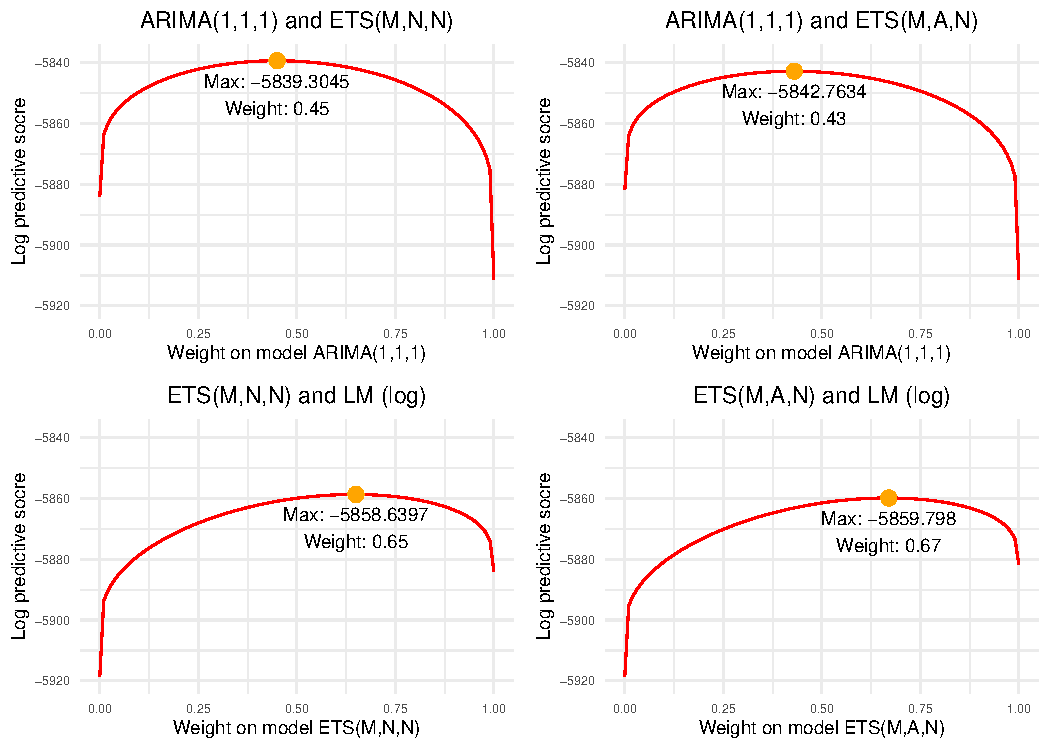
\includegraphics[width=9cm]{Graph/best4comb.pdf}\\
{\tiny{The top four log predictive scores of weighted two-model-pool combinations for S\&P 500 returns.}}
\end{figure}

\end{frame}



\section{Pure Cross-sectional Analysis}

\begin{frame}{Model Setup - True DGP}

\Large
\[y_i = \beta_1 x_{1i} + \beta_2 x_{2i} + \epsilon_i, \ \ \epsilon_i \stackrel{i.i.d}{\sim} N(0,\sigma^2_{\epsilon})\]

\vspace{5mm}
\normalsize
\begin{itemize}
    \item $E[x_{1i}] = E[x_{2i}] = 0$, $Var(x_{1i}) = Var(x_{2i}) = 1$
    \item $Cov(x_{1i}, x_{2i}) = 0.3$ exogenous and weakly correlated regressors
    \item $\pmb{\beta} = (\beta_1, \beta_2)' = (2,2)'$, $\sigma^2_{\epsilon}=4$
    \item All classical assumptions
    \vspace{3mm}
    \item Obtain $y$, $x_{1i}$ and $x_{2i}$
\end{itemize}

\end{frame}



\begin{frame}{Model Setup - Forecasting Models}

The constituent models in matrix form are proposed as
\Large
\begin{align*}
M_1 : y &= x_1 \alpha_{1} + u_1, \ \ u_{1} \stackrel{i.i.d}{\sim} N(0,\sigma^2_1) \\
M_2 : y &= x_2 \alpha_{2} + u_2, \ \ u_{2} \stackrel{i.i.d}{\sim} N(0,\sigma^2_2).
\end{align*}
\normalsize
\begin{itemize}
    \item Obtain $\hat y_{1}$ from $M_1$ and $\hat y_{2}$ from $M_2$
    \vspace{3mm}
    \item Aggregate them linearly $\hat y = \hat y_{1}\omega + \hat y_{2}(1-\omega)$
\end{itemize}

\end{frame}



\begin{frame}{Optimal Weight Derivation - Minimization}

The optimal weight is obtained over the in-sample period (R).
\vspace{-1mm}
\begin{align*}
\hat{\omega}_{\text{opt}} 
&= \underset{\omega \in [0,1]}{\arg\min} \ \frac{1}{R} \sum^R_{t=1} \Big[y - \big(\hat y_{1} \omega + \hat y_{2} (1-\omega)\big)\Big]' \Big[y - \big(\hat y_{1} \omega + \hat y_{2} (1-\omega)\big)\Big] \\
&= \underset{\omega \in [0,1]}{\arg\min} \ \frac{1}{R} \sum^R_{t=1} \Big[y - \big(x_1 \hat\alpha_1 \omega + \ x_2 \hat\alpha_2 (1-\omega)\big)\Big]'\Big[y - \big(x_1 \hat\alpha_1 \omega + \ x_2 \hat\alpha_2 (1-\omega)\big)\Big] \\
&= \underset{\omega \in [0,1]}{\arg\min} \ \frac{1}{R} \sum^R_{t=1} \big[y-(x_1 \hat\alpha_1 - x_2 \hat\alpha_2) \omega - x_2 \hat\alpha_2\big]'\big[y-(x_1 \hat\alpha_1 - x_2 \hat\alpha_2) \omega - x_2 \hat\alpha_2\big]
\end{align*}

\onslide<2-> \[-2(x_1 \hat\alpha_1 - x_2 \hat\alpha_2)' (y-(x_1 \hat\alpha_1 - x_2 \hat\alpha_2) \hat\omega_{opt} - x_2 \hat\alpha_2) = 0\]

\end{frame}



\begin{frame}{Optimal Weight Derivation - Findings}

\begin{align*}
\hat\omega_{opt} 
&= \frac{(x_1 \hat\alpha_1 - x_2 \hat\alpha_2)' y - (x_1 \hat\alpha_1 - x_2 \hat\alpha_2)' x_2 \hat\alpha_2}{\hat\alpha'_1 x'_1 x_1 \hat\alpha_1 - 2\hat\alpha'_1 x'_1 x_2 \hat\alpha_2 + \hat\alpha'_2 x'_2 x_2 \hat\alpha_2} \\
&= \frac{\alt<1>{\alert{\hat\alpha_1'}}{\hat\alpha_1'}\alt<2>{\alert{\text{cov}_R(x_1,x_1)}}{\text{cov}_R(x_1,x_1)}\alt<1>{\alert{\hat\alpha_1}}{\hat\alpha_1} - \alt<1>{\alert{\hat\alpha_1'}}{\hat\alpha_1'}\alt<3>{\alert{\text{cov}_R(x_1,x_2)}}{\text{cov}_R(x_1,x_2)}\alt<1>{\alert{\hat\alpha_2}}{\hat\alpha_2}}{\alt<1>{\alert{\hat\alpha_1'}}{\hat\alpha_1'} \alt<2>{\alert{\text{cov}_R(x_1,x_1)}}{\text{cov}_R(x_1,x_1)}\alt<1>{\alert{\hat\alpha_1}}{\hat\alpha_1} - 2\alt<1>{\alert{\hat\alpha_1'}}{\hat\alpha_1'}\alt<3>{\alert{\text{cov}_R(x_1,x_2)}}{\text{cov}_R(x_1,x_2)}\alt<1>{\alert{\hat\alpha_2}}{\hat\alpha_2} + \alt<1>{\alert{\hat\alpha_2'}}{\hat\alpha_2'}\alt<2>{\alert{\text{cov}_R(x_1,x_1)}}{\text{cov}_R(x_2,x_2)}\alt<1>{\alert{\hat\alpha_2}}{\hat\alpha_2}}
\end{align*}

\vspace{3mm}

The estimated optimal weight $\hat\omega_{opt}$ is affected by
    \begin{enumerate}[<+->]
        \item the magnitude of estimated coefficient(s) in each constituent model 
        \item the variances of regressors
        \item the covariance of regressors 
    \end{enumerate}

\end{frame}



\begin{frame}{Optimal Weight Derivation - Limiting Result}
\[\hat\omega_{opt} \overset{p}{\to} \omega_\star 
    = \frac{\alpha_1'\Sigma_{11}\alpha_1 - \alpha_1'\Sigma_{12}\alpha_2}{\alpha_1'\Sigma_{11}\alpha_1 - 2\alpha_1'\Sigma_{12}\alpha_2 + \alpha_2'\Sigma_{22}\alpha_2}\]

\vspace{3mm}

For $\omega_\star = \frac{1}{2}$, it must be that 
\[\alpha_1'\Sigma_{11}\alpha_1 = \alpha_2'\Sigma_{22}\alpha_2.\]

\vspace{3mm}

Asymptotically, any situation where this final equality is nearly satisfied will inevitably lead the optimal weight to be around a half.
\end{frame}



\begin{frame}[plain]
    \begin{figure}
        \centering
        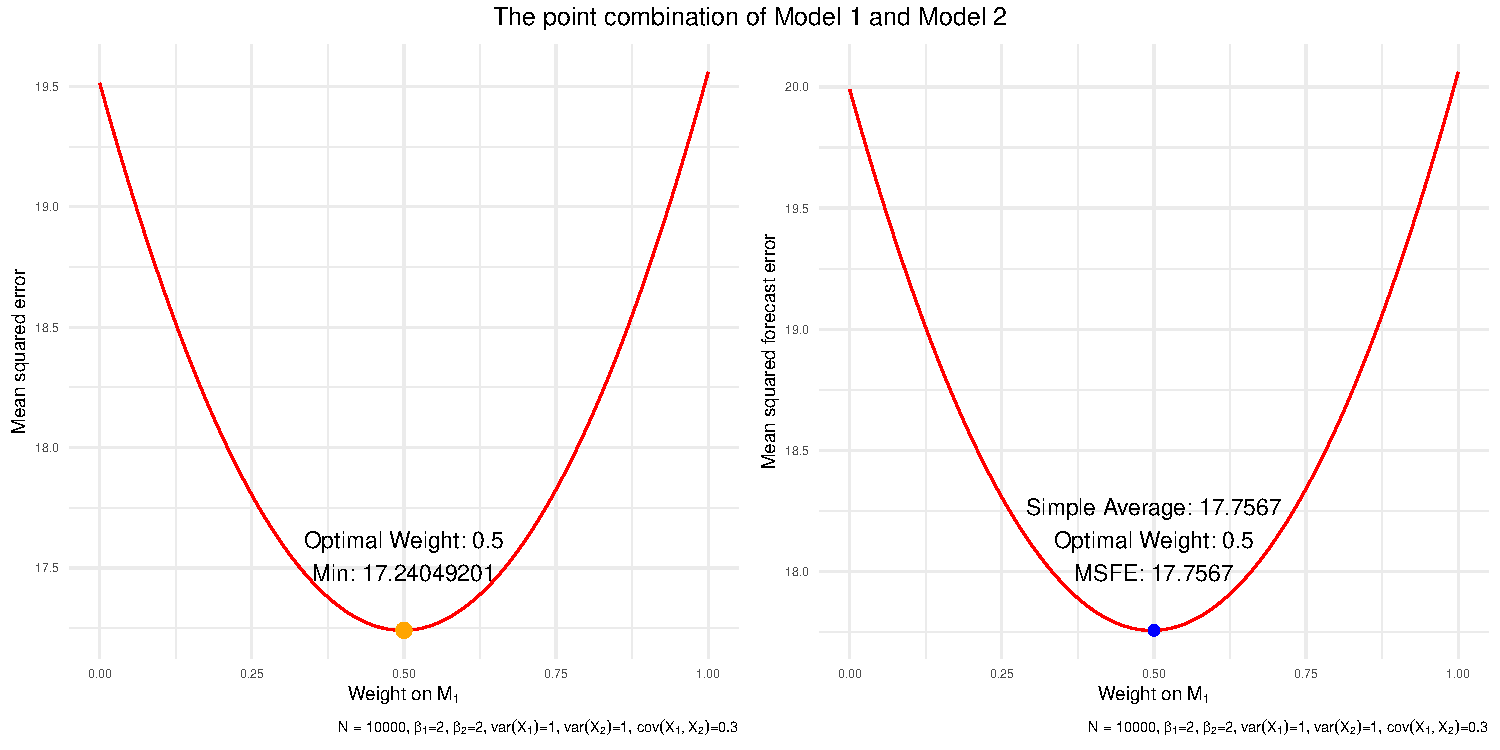
\includegraphics[scale=0.55]{Graph/MSFE.pdf}
        \caption{\footnotesize{$\hat\omega_{opt}$ = 0.5, \alert{N = 10000}, $\beta_1$=2, $\beta_2$=2, $var(X_1)$=1, $var(X_2)$=1, $cov(X_1,X_2)$=0.3}}
    \end{figure}
\end{frame}



\begin{frame}{Density Simulations}
    Applying the learning to density combinations 
    
    \begin{itemize}
        \item Log scoring rules
        \item No closed-form expression
        \item Applicability of findings
    \end{itemize}

\end{frame}



\begin{frame}[plain]
    \begin{figure}
        \centering
        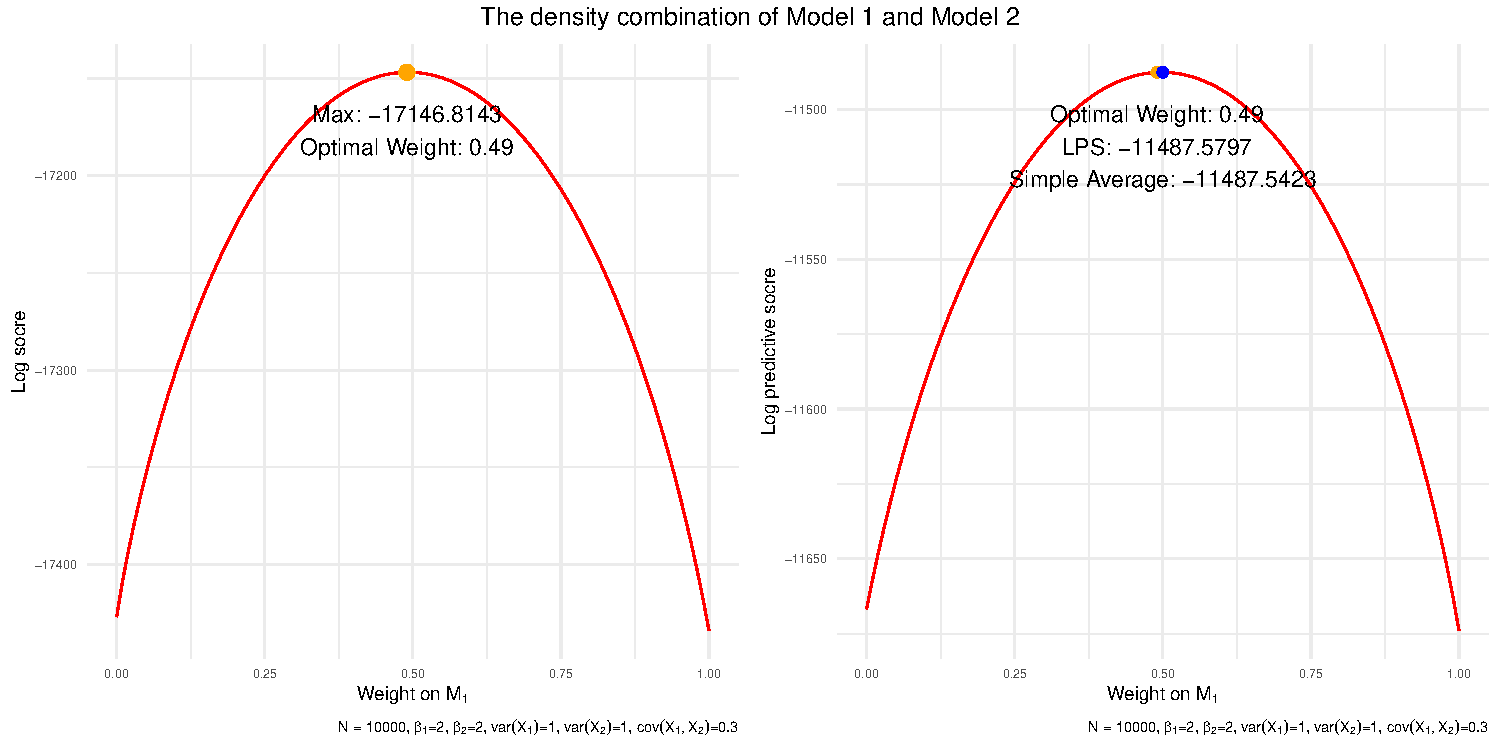
\includegraphics[scale=0.55]{Graph/LPS_10000.pdf}
        \caption{\footnotesize{$\hat\omega_{opt}$ = 0.49, N = 10000, $\beta_1$=2, $\beta_2$=2, $var(X_1)$=1, $var(X_2)$=1, $cov(X_1,X_2)$=0.3}}
    \end{figure}
\end{frame}



\begin{frame}[plain]
    \begin{figure}
        \centering
        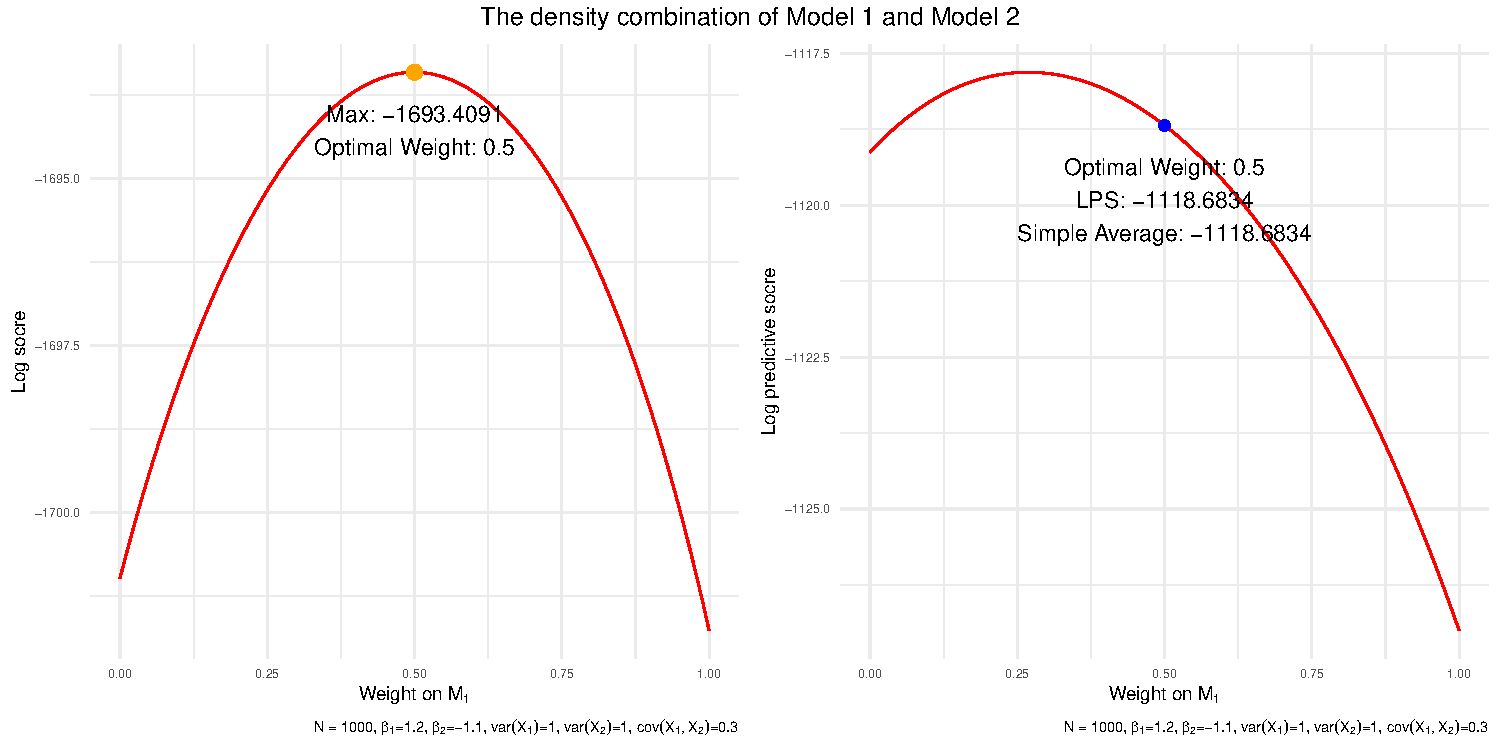
\includegraphics[scale=0.55]{Graph/LPS_1000.pdf}
        \caption{\footnotesize{\alert{$\hat\omega_{opt}$ = 0.5}, N = 1000, \alert{$\beta_1$=1.2}, \alert{$\beta_2$=-1.1}, $var(X_1)$=1, $var(X_2)$=1, $cov(X_1,X_2)$=0.3}}
    \end{figure}
\end{frame}



\begin{frame}[plain]
    \begin{figure}
        \centering
        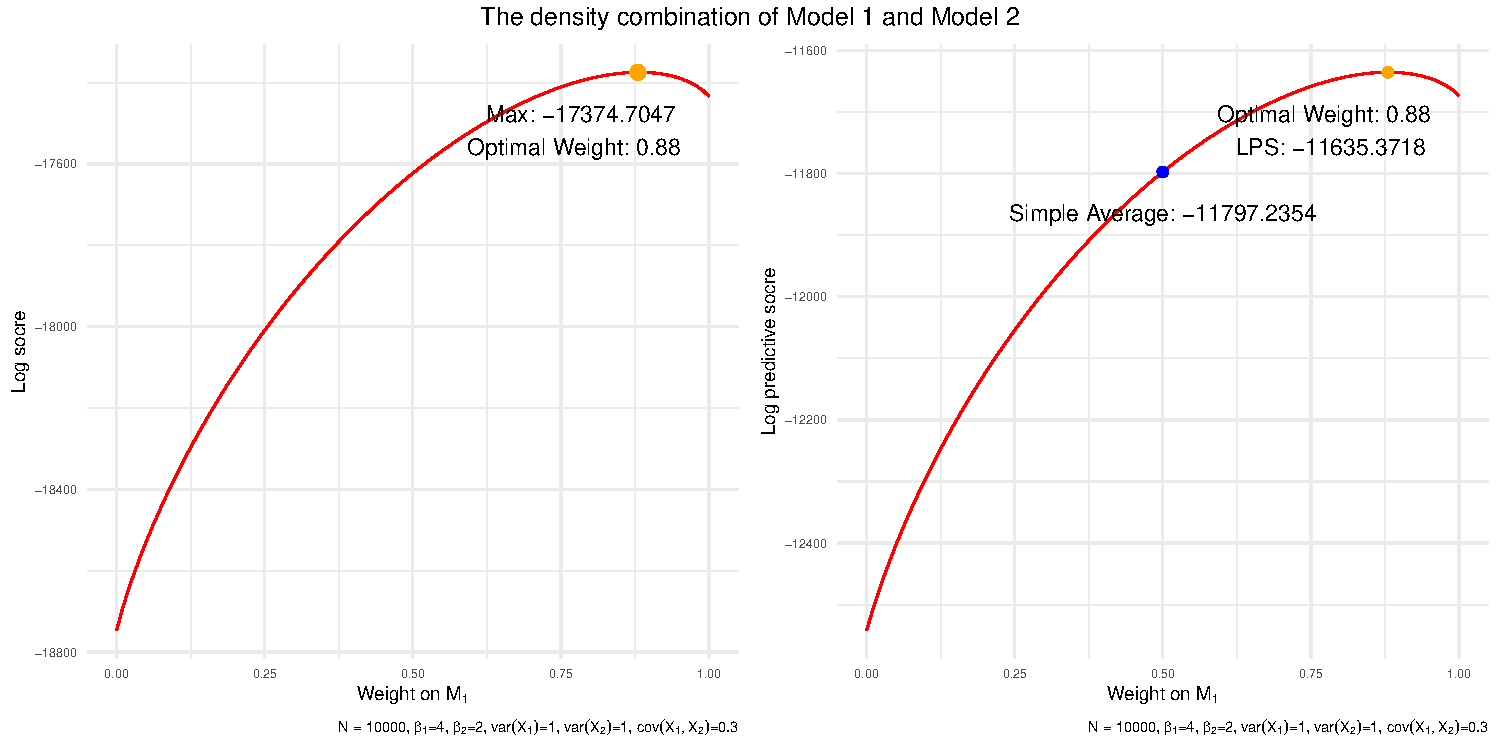
\includegraphics[scale=0.55]{Graph/LPS_1.pdf}
        \caption{\footnotesize{\alert{$\hat\omega_{opt}$ = 0.88}, N = 10000, \alert{$\beta_1$=4}, \alert{$\beta_2$=2}, $var(X_1)$=1, $var(X_2)$=1, $cov(X_1,X_2)$=0.3}}
    \end{figure}
\end{frame}



\begin{frame}[plain]
    \begin{figure}
        \centering
        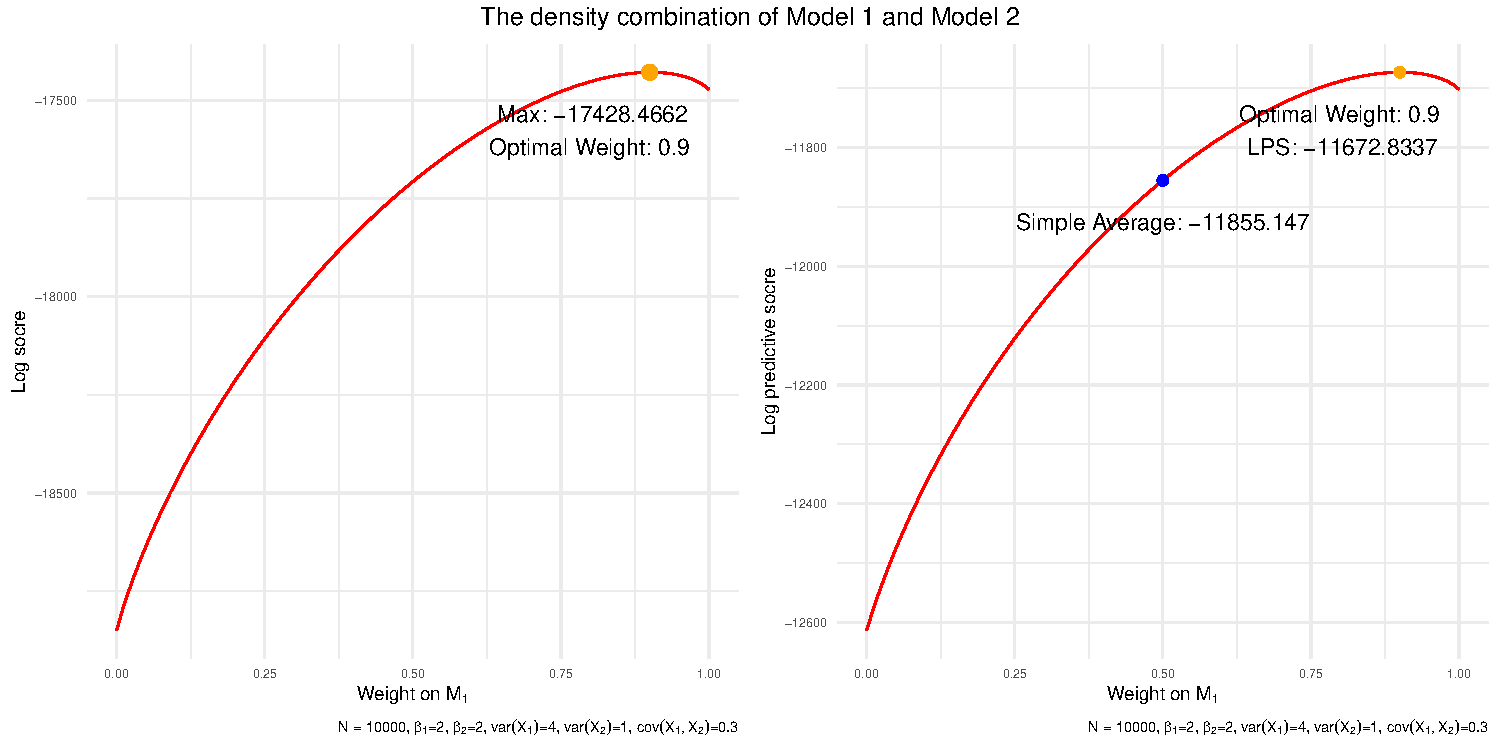
\includegraphics[scale=0.55]{Graph/LPS_2.pdf}
        \caption{\footnotesize{\alert{$\hat\omega_{opt}$ = 0.9}, N = 10000, $\beta_1$=2, $\beta_2$=2, \alert{$var(X_1)$=4}, \alert{$var(X_2)$=1}, $cov(X_1,X_2)$=0.3}}
    \end{figure}
\end{frame}







\section{Conclusion}

\begin{frame}
	\frametitle{Conclusion}
 
 Forecast combinations can deliver improved accuracy over single models, but are not necessarily superior to forecasts obtained from the equally weighted combination.

\end{frame}


\begin{frame}
	\frametitle{Timeline}
 
 \begin{table}[htbp]
  \centering
    \begin{tabular}{ll}
    Time  & Objectives \\
    \midrule
    May - June & Investigating the presence of puzzle in \\
               & panel data and literature review \\
    \midrule
    July - August & Applying the forecast accuracy tests with \\
                  & time series data and drafting thesis  \\
    \midrule
    September & Attempting the tests with panel data and \\
              & considering limitations \\
    \midrule
    October & Working on the thesis and presentation \\
    \bottomrule
    \end{tabular}
\end{table}


\end{frame}


\begin{frame}

     \begin{center}
        {\Huge\atchen Thank You!}
    \end{center}
    
    \bigskip
    
    \begin{center}
            {\LARGE Questions?}
    \end{center}
    
\end{frame}


% Remove headers from top
\appendix
\setbeamertemplate{headline}{
    \nointerlineskip
}
\addtobeamertemplate{frametitle}{\vspace*{-\headheight}}{}

\begin{frame}[noframenumbering, allowframebreaks]
    \frametitle{References}
    \printbibliography[title={References}, heading=bibintoc, style=apa]
\end{frame}


\begin{frame}

     \begin{center}
        {\Huge\atchen Thank You!}
    \end{center}
    
    \bigskip
    
    \begin{center}
            {\LARGE Questions?}
    \end{center}
    
\end{frame}

\section{Appendix}

\begin{frame}{Example 1 (Nonstationary) - Model Specification I}
    
    \begin{itemize}
    \item ARIMA(1,1,1) model 
        \begin{equation*}
        log(y_t) = c + log(y_{t-1}) + \phi_1\big[log(y_{t-1})-log(y_{t-2})\big] + \epsilon_t + \theta_1\epsilon_{t-1}
        \end{equation*}
        
    \item ETS(M,N,N) model
        \begin{align*}
        y_t &= \ell_{t-1} (1+\epsilon_t) \\
        \ell_t &= \ell_{t-1} (1+\alpha \epsilon_t) \\
        \end{align*}
    \end{itemize}

\end{frame}



\begin{frame}{Example 1 (Nonstationary) - Model Specification II}

    \begin{itemize}
    \item A linear regression model of the natural logarithm of the S\&P 500 index and ARIMA(1,0,0) errors.
        \begin{align*}
        log(y_t) &= \beta_0 + \beta_1 t + u_t \\
        u_t &= \phi_1 u_{t-1} + \epsilon_t
        \end{align*}
    \end{itemize}

The $\epsilon_t$ in each model is assumed to be independent and normally distributed with a zero mean and a constant variance.

\end{frame}



\begin{frame}{Example 1 (Stationary) - Model Specification}

    \begin{itemize}
    \item ARMA(1,1) model with an intercept of the natural logarithm of S\&P 500 returns. 
        \begin{equation*}
    log(y_t) - log(y_{t-1}) = c + \phi_1\big[log(y_{t-1})-log(y_{t-2})\big] + \epsilon_t + \theta_1\epsilon_{t-1}
    \end{equation*}

    \item A classical linear regression model of the natural logarithm of the S\&P 500 returns and ARMA(1,1) errors. 
    \begin{align*}
    log(y_t) &= \beta_0 + u_t \\
    u_t &= \phi_1 u_{t-1} + \epsilon_t + \theta_1\epsilon_{t-1}
    \end{align*}
    \end{itemize}
    
\end{frame}



\begin{frame}{Example 2 - Well-specified Models}

    \begin{itemize}
    \item ARIMA(2,0,2)(0,1,1)[4] model with an intercept of the natural logarithm of unemployed individuals.
    \begin{align*}
    log(y_t) &= c + log(y_{t-4}) + \phi_1\big[log(y_{t-1})-log(y_{t-5})\big] \\
    & + \phi_2\big[log(y_{t-2})-log(y_{t-6})\big] + \epsilon_t + \theta_1\epsilon_{t-1} + \theta_2\epsilon_{t-2} \\
    & + \Theta_1\epsilon_{t-4} + \theta_1\Theta_1\epsilon_{t-5} + \theta_2\Theta_1\epsilon_{t-6} \\
    \end{align*}

    \vspace{-5mm}

    \item ETS(A,A,A) model of the natural logarithm of unemployed individuals. 
    \begin{align*}
    log(y_t) &= \ell_{t-1} + b_{t-1} + s_{t-m} + \epsilon_t \\
    \ell_t &= \ell_{t-1} + b_{t-1} + \alpha \epsilon_t \\
    b_t &= b_{t-1} + \beta \epsilon_t \\
    s_{t} &= s_{t-m} + \gamma \epsilon_t
    \end{align*}
    \end{itemize}
    
\end{frame}



\begin{frame}{Example 2 - Poorly-specified Models}

    \begin{itemize}
    \item ARIMA(2,1,0) model with an intercept of the natural logarithm of unemployed individuals.
    \begin{equation*}
    log(y_t) = c + log(y_{t-1}) + \phi_1\big[log(y_{t-1})-log(y_{t-2})\big] + \phi_2\big[log(y_{t-2})-log(y_{t-3})\big] + \epsilon_t
    \end{equation*}

    \item ETS(A,A,N) model of the natural logarithm of unemployed individuals. 
    \begin{align*}
    log(y_t) &= \ell_{t-1} + b_{t-1} + \epsilon_t \\
    \ell_t &= \ell_{t-1} + b_{t-1} + \alpha \epsilon_t \\
    b_t &= b_{t-1} + \beta \epsilon_t
    \end{align*}
    \end{itemize}
    
\end{frame}



\begin{frame}{Optimal Weight Derivation (Detail) - Model}

    Models can be written in matrix forms
\[y = x_1 \beta_{1} + x_2 \beta_{2} + \epsilon\]
\[ M_1 : y = x_1 \alpha_{1} + u_1\]
\[ M_2 : y = x_2 \alpha_{2} + u_2\]

where
\[
     {y}=\begin{bmatrix}
           y_{1} \\
           y_{2} \\
           \vdots \\
           y_{N}
         \end{bmatrix},\;
     {x_1}=\begin{bmatrix}
           x_{11} \\
           x_{21} \\
           \vdots \\
           x_{N1}
         \end{bmatrix},\;
    {x_2}=\begin{bmatrix}
           x_{12} \\
           x_{22} \\
           \vdots \\
           x_{N2}
         \end{bmatrix},\;
    {\epsilon}=\begin{bmatrix}
           \epsilon_{1} \\
           \epsilon_{2} \\
           \vdots \\
           \epsilon_{N}
         \end{bmatrix}.
\]

\end{frame}



\begin{frame}{Optimal Weight Derivation (Detail) - Parameter Estimation}
    Applying the OLS estimation.
\vspace{-0.2mm}
\begin{align*}
    \hat\alpha_{1} &= (x'_1x_1)^{-1} x'_1y \\
    &= (x'_1x_1)^{-1} x'_1(x_1 \beta_{10} + x_2 \beta_{20} + \epsilon) \\
    &= \beta_{10} + (x'_1x_1)^{-1} x'_1x_2 \beta_{20} \\
    &= \beta_{10} + var(x_1)^{-1} cov(x_1,x_2) \beta_{20} \\
    \\
    \hat\alpha_{2} &= (x'_2x_2)^{-1} x'_2y \\
    &= (x'_2x_2)^{-1} x'_2(x_1 \beta_{10} + x_2 \beta_{20} + \epsilon) \\
    &= \beta_{20} + (x'_2x_2)^{-1} x'_2x_1 \beta_{10} \\
    &= \beta_{20} + var(x_2)^{-1} cov(x_2,x_1) \beta_{10} \\
\end{align*}
    
\end{frame}


\begin{frame}{Optimal Weight Derivation (Detail) - MSE}

\begin{align*}
    \hat y &= \hat y_1 \omega + \hat y_2 (1-\omega) \\
    &= x_1 \hat\alpha_1 \omega + \ x_2 \hat\alpha_2 (1-\omega) \\
    &= x_1 \hat\alpha_1 \omega - x_2 \hat\alpha_2 \omega + x_2 \hat\alpha_2 \\
    &= (x_1 \hat\alpha_1 - x_2 \hat\alpha_2) \omega + x_2 \hat\alpha_2
\end{align*}
\begin{align*}
\hat{\omega}_{\text{opt}} 
&= \underset{\omega \in [0,1]}{\arg\min} E\big[(Y - \hat Y)' (Y - \hat Y) \big] \\
&= \underset{\omega \in [0,1]}{\arg\min} \ E\bigg\{\big[Y-(x_1 \hat\alpha_1 - x_2 \hat\alpha_2) \omega - x_2 \hat\alpha_2\big]'\big[Y-(x_1 \hat\alpha_1 - x_2 \hat\alpha_2) \omega - x_2 \hat\alpha_2\big]\bigg\}
\end{align*}
\end{frame}



\begin{frame}{Optimal Weight Derivation (Detail) - Optimal Weight}
Solve the First-order condition
\[-2(x_1 \hat\alpha_1 - x_2 \hat\alpha_2)' (y-(x_1 \hat\alpha_1 - x_2 \hat\alpha_2) \hat\omega_{opt} - x_2 \hat\alpha_2) = 0.\]
\begin{align*}
    (x_1 \hat\alpha_1 - x_2 \hat\alpha_2)' (x_1 \hat\alpha_1 - x_2 \hat\alpha_2) \hat\omega_{opt} &= (x_1 \hat\alpha_1 - x_2 \hat\alpha_2)' (y - x_2 \hat\alpha_2) \\
    \hat\omega_{opt} &= \frac{(x_1 \hat\alpha_1 - x_2 \hat\alpha_2)' (y - x_2 \hat\alpha_2)}{(x_1 \hat\alpha_1 - x_2 \hat\alpha_2)' (x_1 \hat\alpha_1 - x_2 \hat\alpha_2)} \\
    \hat\omega_{opt} &= \frac{(x_1 \hat\alpha_1 - x_2 \hat\alpha_2)' (y - x_2 \hat\alpha_2)}{(x_1 \hat\alpha_1 - x_2 \hat\alpha_2)' (x_1 \hat\alpha_1 - x_2 \hat\alpha_2)} \\
    \hat\omega_{opt} &= \frac{(x_1 \hat\alpha_1 - x_2 \hat\alpha_2)' y - (x_1 \hat\alpha_1 - x_2 \hat\alpha_2)' x_2 \hat\alpha_2}{\hat\alpha'_1 x'_1 x_1 \hat\alpha_1 - 2\hat\alpha'_1 x'_1 x_2 \hat\alpha_2 + \hat\alpha'_2 x'_2 x_2 \hat\alpha_2} \\
\end{align*}
\end{frame}



\begin{frame}{Optimal Weight Derivation (Detail) - Meaningful Expression}
\begin{align*}
  \hat\omega_{opt} 
    &= \frac{R^{-1}(x_1 \hat\alpha_1 - x_2 \hat\alpha_2)' y - R^{-1}(x_1 \hat\alpha_1 - x_2 \hat\alpha_2)' x_2 \hat\alpha_2}{\hat\alpha'_1 \frac{x'_1 x_1}{R} \hat\alpha_1 - 2\hat\alpha'_1 \frac{x'_1 x_2}{R} \hat\alpha_2 + \hat\alpha'_2 \frac{x'_2 x_2}{R} \hat\alpha_2} \\
    &= \frac{\hat\alpha_1' \text{cov}_R(x_1,y)-\hat\alpha_2'\text{cov}_R(x_2,y)-\hat\alpha_1'\text{cov}_R(x_1,x_2)\hat\alpha_2 + \hat\alpha_2'\text{cov}_R(x_2,x_2)\hat\alpha_2}{\hat\alpha_1' \text{cov}_R(x_1,x_1)\hat\alpha_1 - 2\hat\alpha_1'\text{cov}_R(x_1,x_2)\hat\alpha_2 + \hat\alpha_2'\text{cov}_R(x_2,x_2)\hat\alpha_2} \\
    &= \frac{\hat\alpha_1'\text{cov}_R(x_1,x_1)\hat\alpha_1 - \hat\alpha_1'\text{cov}_R(x_1,x_2)\hat\alpha_2}{\hat\alpha_1' \text{cov}_R(x_1,x_1)\hat\alpha_1 - 2\hat\alpha_1'\text{cov}_R(x_1,x_2)\hat\alpha_2 + \hat\alpha_2'\text{cov}_R(x_2,x_2)\hat\alpha_2}
\end{align*}
\end{frame}




\begin{frame}{Optimal Weight Derivation (Detail) - Limit Result}

\[\omega_\star = \frac{\alpha_1'\Sigma_{11}\alpha_1 -\alpha_1'\Sigma_{12}\alpha_2}{\alpha_1'\Sigma_{11}\alpha_1 - 2\alpha_1'\Sigma_{12}\alpha_2 + \alpha_2'\Sigma_{22}\alpha_2}\]

For $\omega_\star=\frac{1}{2}$ it must be that 

\begin{flalign*}
\frac{1}{2} &= \frac{\alpha_1'\Sigma_{11}\alpha_1 -\alpha_1'\Sigma_{12}\alpha_2}{\alpha_1'\Sigma_{11}\alpha_1 - 2\alpha_1'\Sigma_{12}\alpha_2 + \alpha_2'\Sigma_{22}\alpha_2} \\
\alpha_1'\Sigma_{11}\alpha_1 - 2\alpha_1'\Sigma_{12}\alpha_2 + \alpha_2'\Sigma_{22}\alpha_2 &= 2\big(\alpha_1'\Sigma_{11}\alpha_1 -\alpha_1'\Sigma_{12}\alpha_2\big) \\
\alpha_1'\Sigma_{11}\alpha_1 + \alpha_2'\Sigma_{22}\alpha_2 &= 2\alpha_1'\Sigma_{11}\alpha_1 \\
\alpha_1'\Sigma_{11}\alpha_1
&=\alpha_2'\Sigma_{22}\alpha_2.
\end{flalign*}

\end{frame}



\begin{frame}{Optimal Weight Derivation (Detail) - F-statistic}

Define the sum squared of errors (SSE) for the true model is $SSE_{full} = (y - x_1 \hat\beta_1 - x_2 \hat\beta_2)'(y - x_1 \hat\beta_1 - x_2 \hat\beta_2)$.

\vspace{5mm}

The unbiased estimator of the true model variance is $s^2=\frac{SSE_{full}}{R-2}$.

\vspace{5mm}

The optimal weight can also be constructed by the F-statistics of $M_1$ and $M_2$.

\[\hat\omega_{opt} = \frac{F_{\alpha_1}- R \ \hat\alpha_1'\text{cov}_R(x_1,x_2)\hat\alpha_2/s^2}{F_{\alpha_1} + F_{\alpha_2} - 2 R \ \hat\alpha_1'\text{cov}_R(x_1,x_2)\hat\alpha_2/s^2}.\]

\end{frame}



\begin{frame}{Optimal Weight Derivation (Detail) - F-statistic}
The F-statistic follows a F-distribution with degrees of freedom (1,R-2) under $H_0$, which is defined as
\[F_{\alpha_1} = R \ s^{-2} \ \hat\alpha'_1 \text{cov}_R(x_1,x_1) \hat\alpha_1.\]

Similarly, we have 
\[F_{\alpha_2} = R \ s^{-2} \ \hat\alpha'_2 \text{cov}_R(x_2,x_2) \hat\alpha_2 \sim F_{1,R-2} \text{ under  H}_0.\]

\end{frame}















\end{document}
